\chapter{Bearings Faults Diagnostic using Neural Networks}

\chapterintrobox{Vibration condition monitoring are vibtal for many industrial systems, vibration data contains very useful information about health state of the equipment. Nevertheless, gaining insights from vibration signals in real-world applications turns out to be a complex—and in many times, unfruitful—process. This is mainly due to the complexity of the problem. This chapter demonstrates image processing based approach for bearings faults diagnostics and convolutional neural networks.}

\section{Generating data from raw vibration signals}


Figure \ref{fig:cw_bearings_data_generation} shows data generation principal where 1-dimensional vibration signals are converted into 2-dimensional arrays (images) by reshaping chunks of length 4096 into matrices of 64$\times$64. This approach was first proposed in \cite{Wen2018} and used on the same dataset.

\begin{figure}[H]
	\centering
	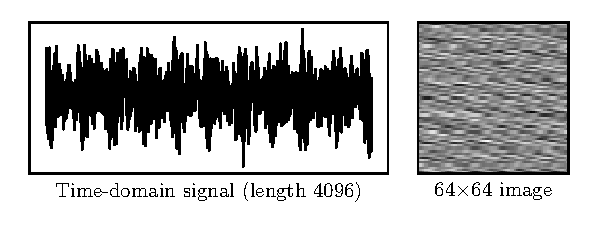
\includegraphics{figures/cw_bearings_data_generation.pdf}
	\caption{Data generation by converting the signal into 64$\times$64 images}
	\label{fig:cw_bearings_data_generation}
\end{figure}



\begin{figure}[H]
    \centering
    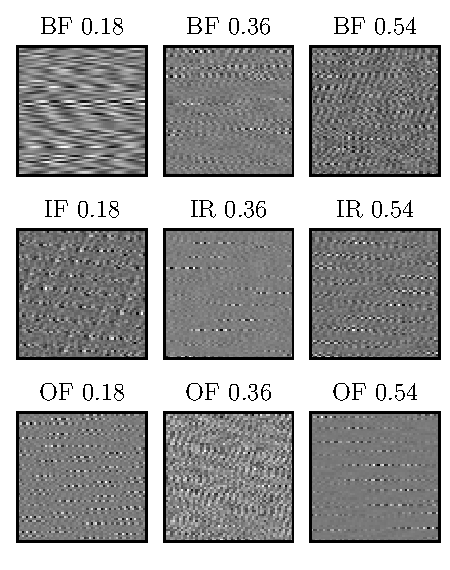
\includegraphics{figures/cw_bearings_faults_samples.pdf}
    \caption{}
    \label{fig:bearings_faults_samples}
\end{figure}

\begin{table}[H]
	\centering
	\begin{tabu}{ll}
		\tabucline[1.5pt]{-} 
	   Class & Samples count \\
	   \hline 
	   Normal bearing & 295 \\
	   Roller element 0.18mm & 146\\
	   Roller element 0.36mm &116\\
	   Roller element 0.54mm&116\\
	   Inner race 0.18mm&295\\
	   Inner race 0.36mm&116\\
	   Inner race 0.54mm&116\\
	   Outer race 0.18mm&116\\
	   Outer race 0.36mm&116\\
	   Outer race 0.54mm&116\\
   \tabucline[1.5pt]{-}
   \end{tabu}
   \caption{}
   \label{table:cw-classes-count}
\end{table}

\section{Bearings faults diagnostic using neural networks}
After generating data by converting raw vibration signals into images, these images serve as an input for a convolutional neural network
\subsection{Network architecture}

\begin{table}[H]
    \centering
    \begin{tabu}{lll}
		\tabucline[1.5pt]{-}
		\textbf{Layer (type)}   & \textbf{Output shape} &   \textbf{Param \#} \\
		\tabucline[1pt]{-}
		Conv1 (Conv2D) 			&   (None, 1, 64 ,32)   &   18464   \\
		MaxPool1 (MaxPool2D) 	&   (None, 1, 32, 32)   &   0       \\
		Conv2 (Conv2D)			&   (None, 1, 32, 64)   &   18496   \\
		MaxPool2 (MaxPooling2D) &   (None, 1, 16, 64)   &   0       \\
		Conv3 (Conv2D)          &   (None, 1, 16, 128)  &   73856   \\
		MaxPool3 (MaxPooling2D) &   (None, 1, 8, 128)   &   0       \\       
		Flatten1 (Flatten)      &   (None, 1024)        &   0       \\     
		Dense1 (Dense)          &   (None, 128)         &   131200  \\   
		Dense2 (Dense)          &   (None, 64)          &   8256    \\     
		Dense3 (Dense)          &   (None, 10)          &   650     \\
		\tabucline[1pt]{-}
		Total params: 250,922       &                   &           \\
		Trainable params: 250,922   &                   &           \\
		Non-trainable params: 0     &                   &           \\
	\tabucline[1.5pt]{-}
    \end{tabu}
    \caption{CNN architecture}
    \label{table:bearings-faults-cnn-classifier-architecture}
\end{table}

\subsection{Training process}

\begin{figure}[H]
    \centering
    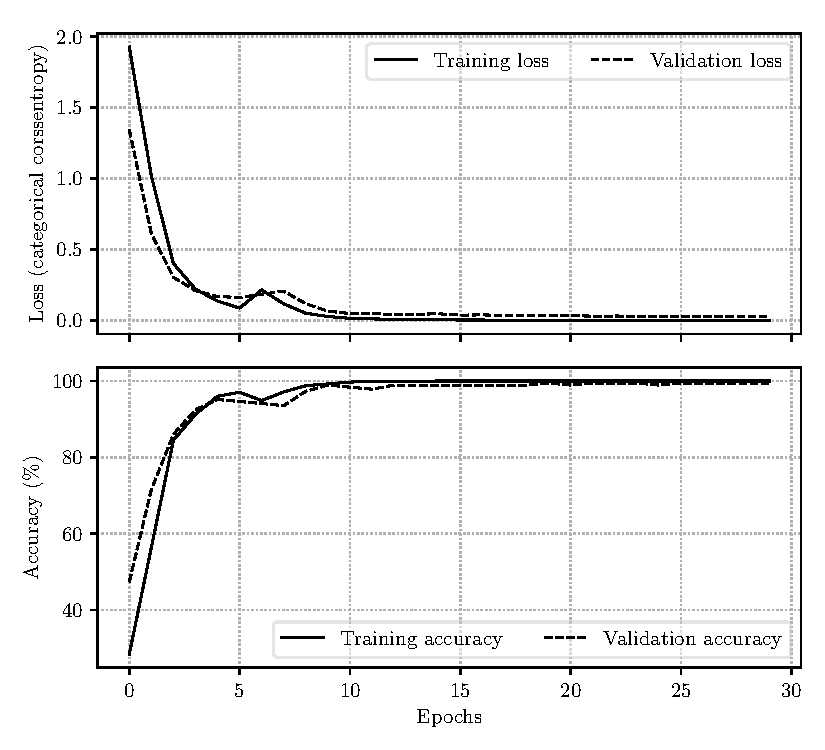
\includegraphics{figures/cw_bearings_faults_classification_training.pdf}
    \caption{Classifier training}
    \label{fig:bearings_faults_classification_training}
\end{figure}

\subsection{Network results discussion}

\begin{table}[H]
	\centering
	\begin{tabu}{lcc}
		\tabucline[1.5pt]{-} 
						&	\textbf{Loss}	&	\textbf{Accuracy}	\\
	   \tabucline[1pt]{-}
		Train set 		&	0.0003			&	100.00\%				\\
		Validation set 	&	0.0269 			&	99.46\%					\\
		Test set		&	0.0586 			&	98.71\%					\\
   \tabucline[1.5pt]{-}
   \end{tabu}
   \caption{}
   \label{table:cw-cnn-results}
\end{table}

\begin{figure}[H]
    \centering
    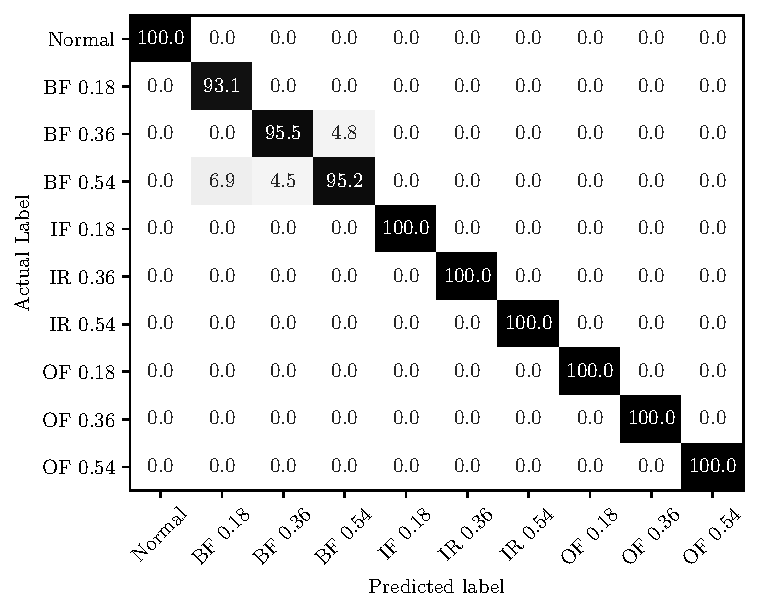
\includegraphics{figures/cw_bearings_faults_classification.pdf}
    \caption{Confusion matrix of bearings faults classification using CNN}
    \label{fig:bearings_faults_classification_confusion_matrix}
\end{figure}

\section{Conclusion}

